\documentclass{beamer}
\bibliographystyle{apalike}

\usetheme{metropolis}           % Use metropolis theme
\title{Supervised Learning of Neural Random-Access Machines with Differential Evolution}
\date{\today}
\author{Valerio Belli}
\institute{Università degli Studi di Perugia}
\titlegraphic{\hfill
\includegraphics[height=1.5cm]{logo.png}}

\begin{document}
  \maketitle
  \section{Neural Random-Access Machines}
  \begin{frame}{What is?}
	It is a machine introduced in \cite{NRAM:2016} based on a neural network which is capable of manipulating pointers and dereferencing them through a ``logical'' circuit. Its objective is to solve a task on which it has been trained creating and executing that circuit.
  \end{frame}
  \begin{frame}{Registers only version}
  	\begin{figure}
  		\centering
  		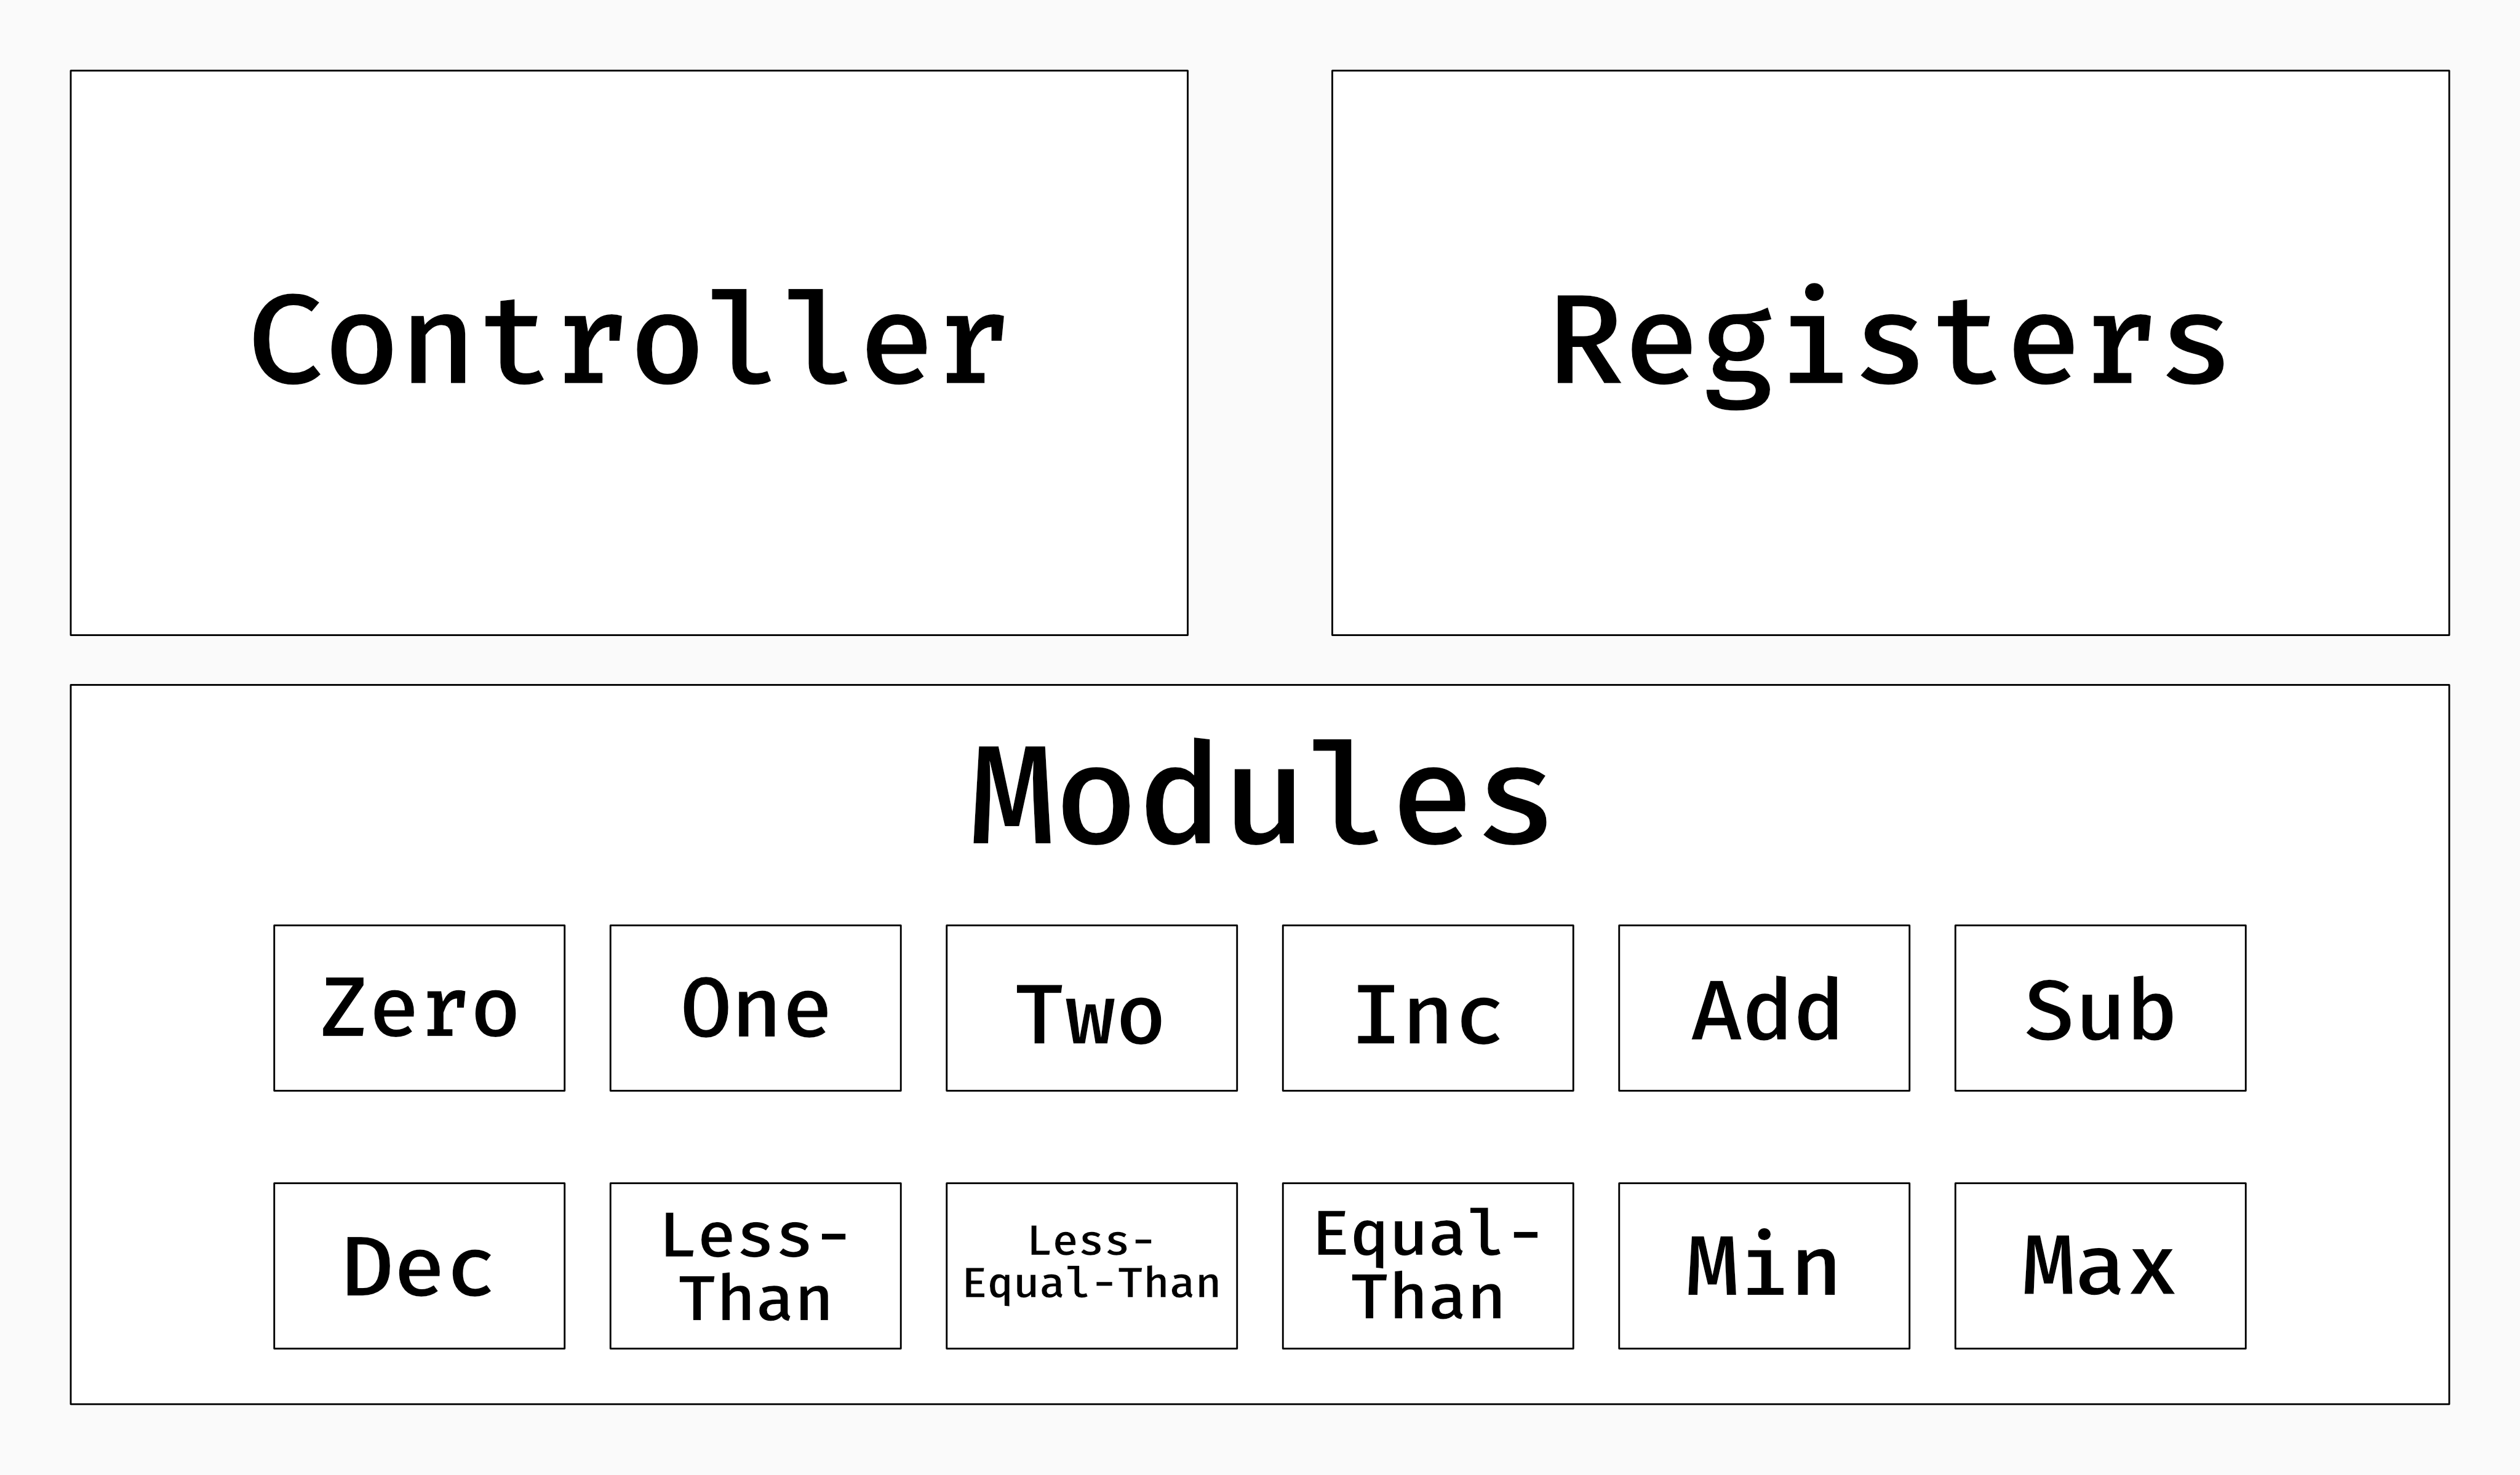
\includegraphics[width=\textwidth]{../figures/schema-nram-without-memory.png}
  	\end{figure}
  \end{frame}
  \begin{frame}{Introduction}
  	Let $N = \{ 1, \dots, I - 1 \}$, where $I$ is an integer constant, the integers set over the NRAM should work. Since the training in \cite{NRAM:2016} is made through a gradient descent algorithm, the NRAM does not work directly over N but over stochastically independent probability distributions, defined as $p \in \mathbb{R}^{I}$ satisfying $0 \leq p_i \leq 1$ and $\sum\limits_{i=0}^{I - 1} p_i = 1$. 
  \end{frame}
  \begin{frame}{Modules}
  	\begin{figure}
  		\centering
  		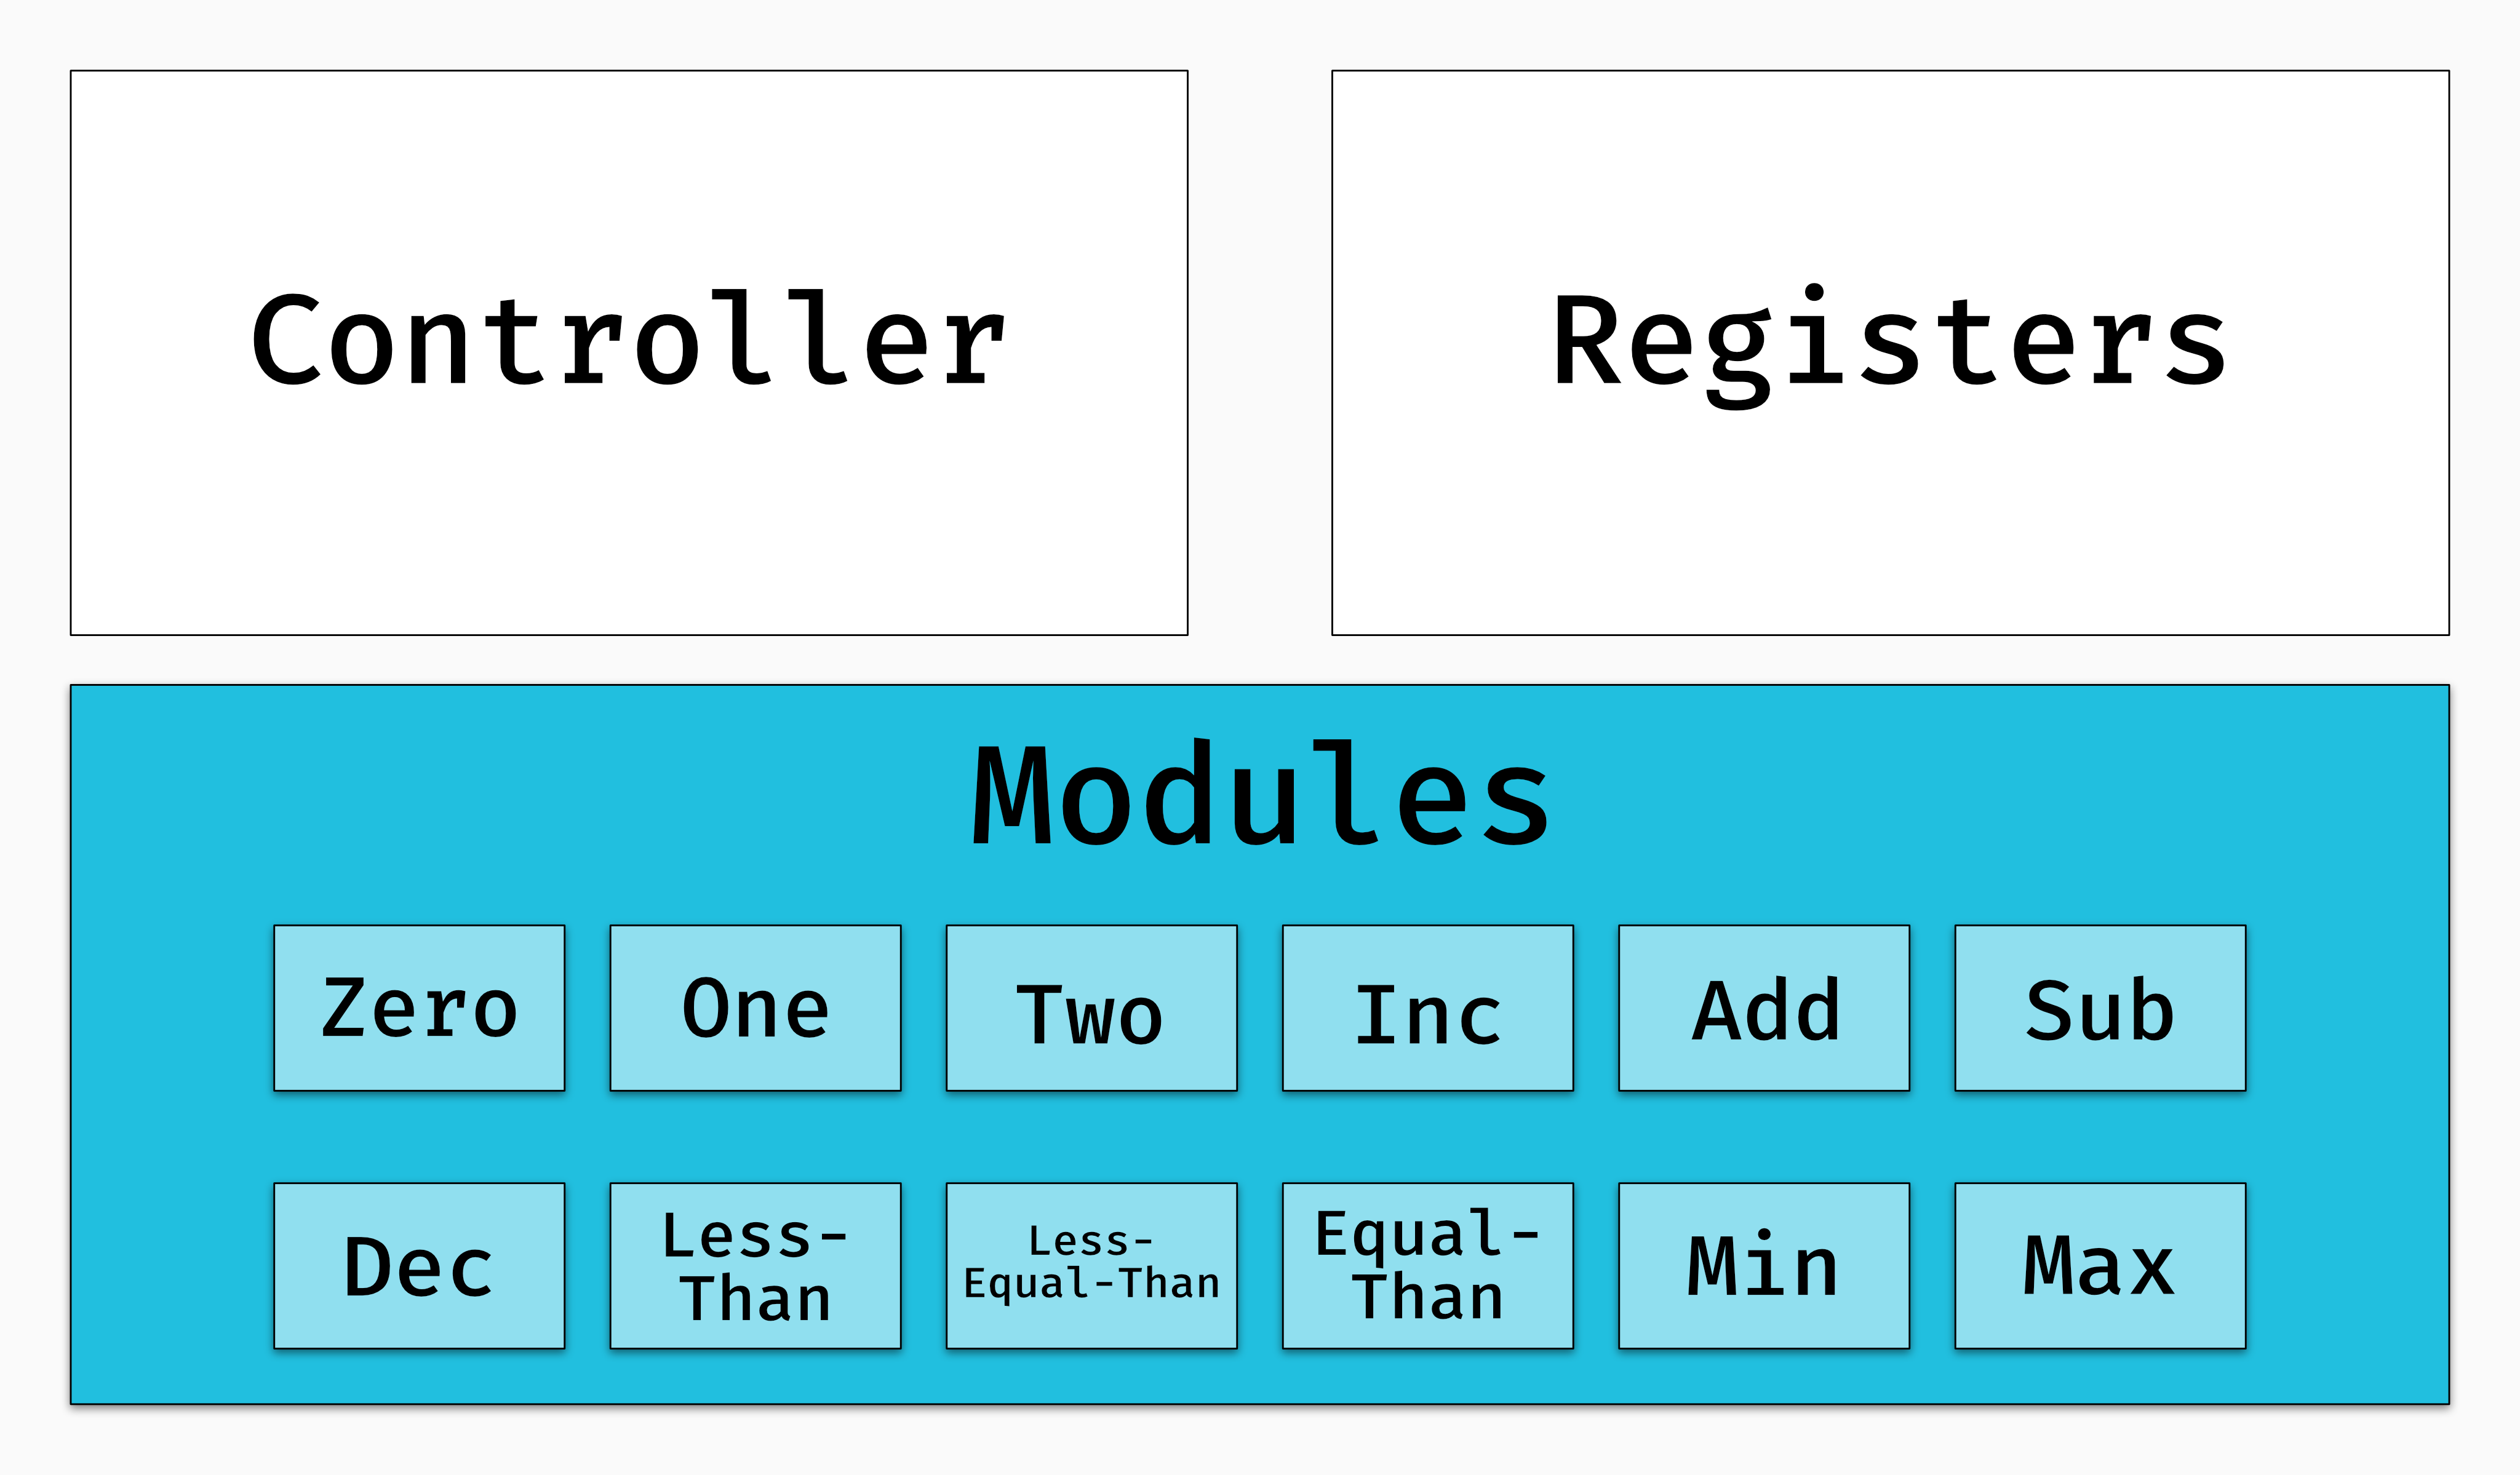
\includegraphics[width=\textwidth]{../figures/schema-nram-without-memory-MS.png}
  	\end{figure}
  \end{frame}
  \begin{frame}{Modules}
  	The modules (or gates) are components through which the controller, connecting them, manipulates values and pointers. In the NRAM exist three types of modules, defined as follows:
  	\begin{align}
		m_i \in N & \textrm{ (Constant modules)} \\
		m_i: p \rightarrow p & \textrm{ (Unary modules)} \\
		m_i: p \times p \rightarrow p & \textrm{ (Binary modules)}
	\end{align}
	Each of them take as input, except the constant modules, and emit probability distributions.
  \end{frame}
  \begin{frame}{Registers}
  	\begin{figure}
  		\centering
  		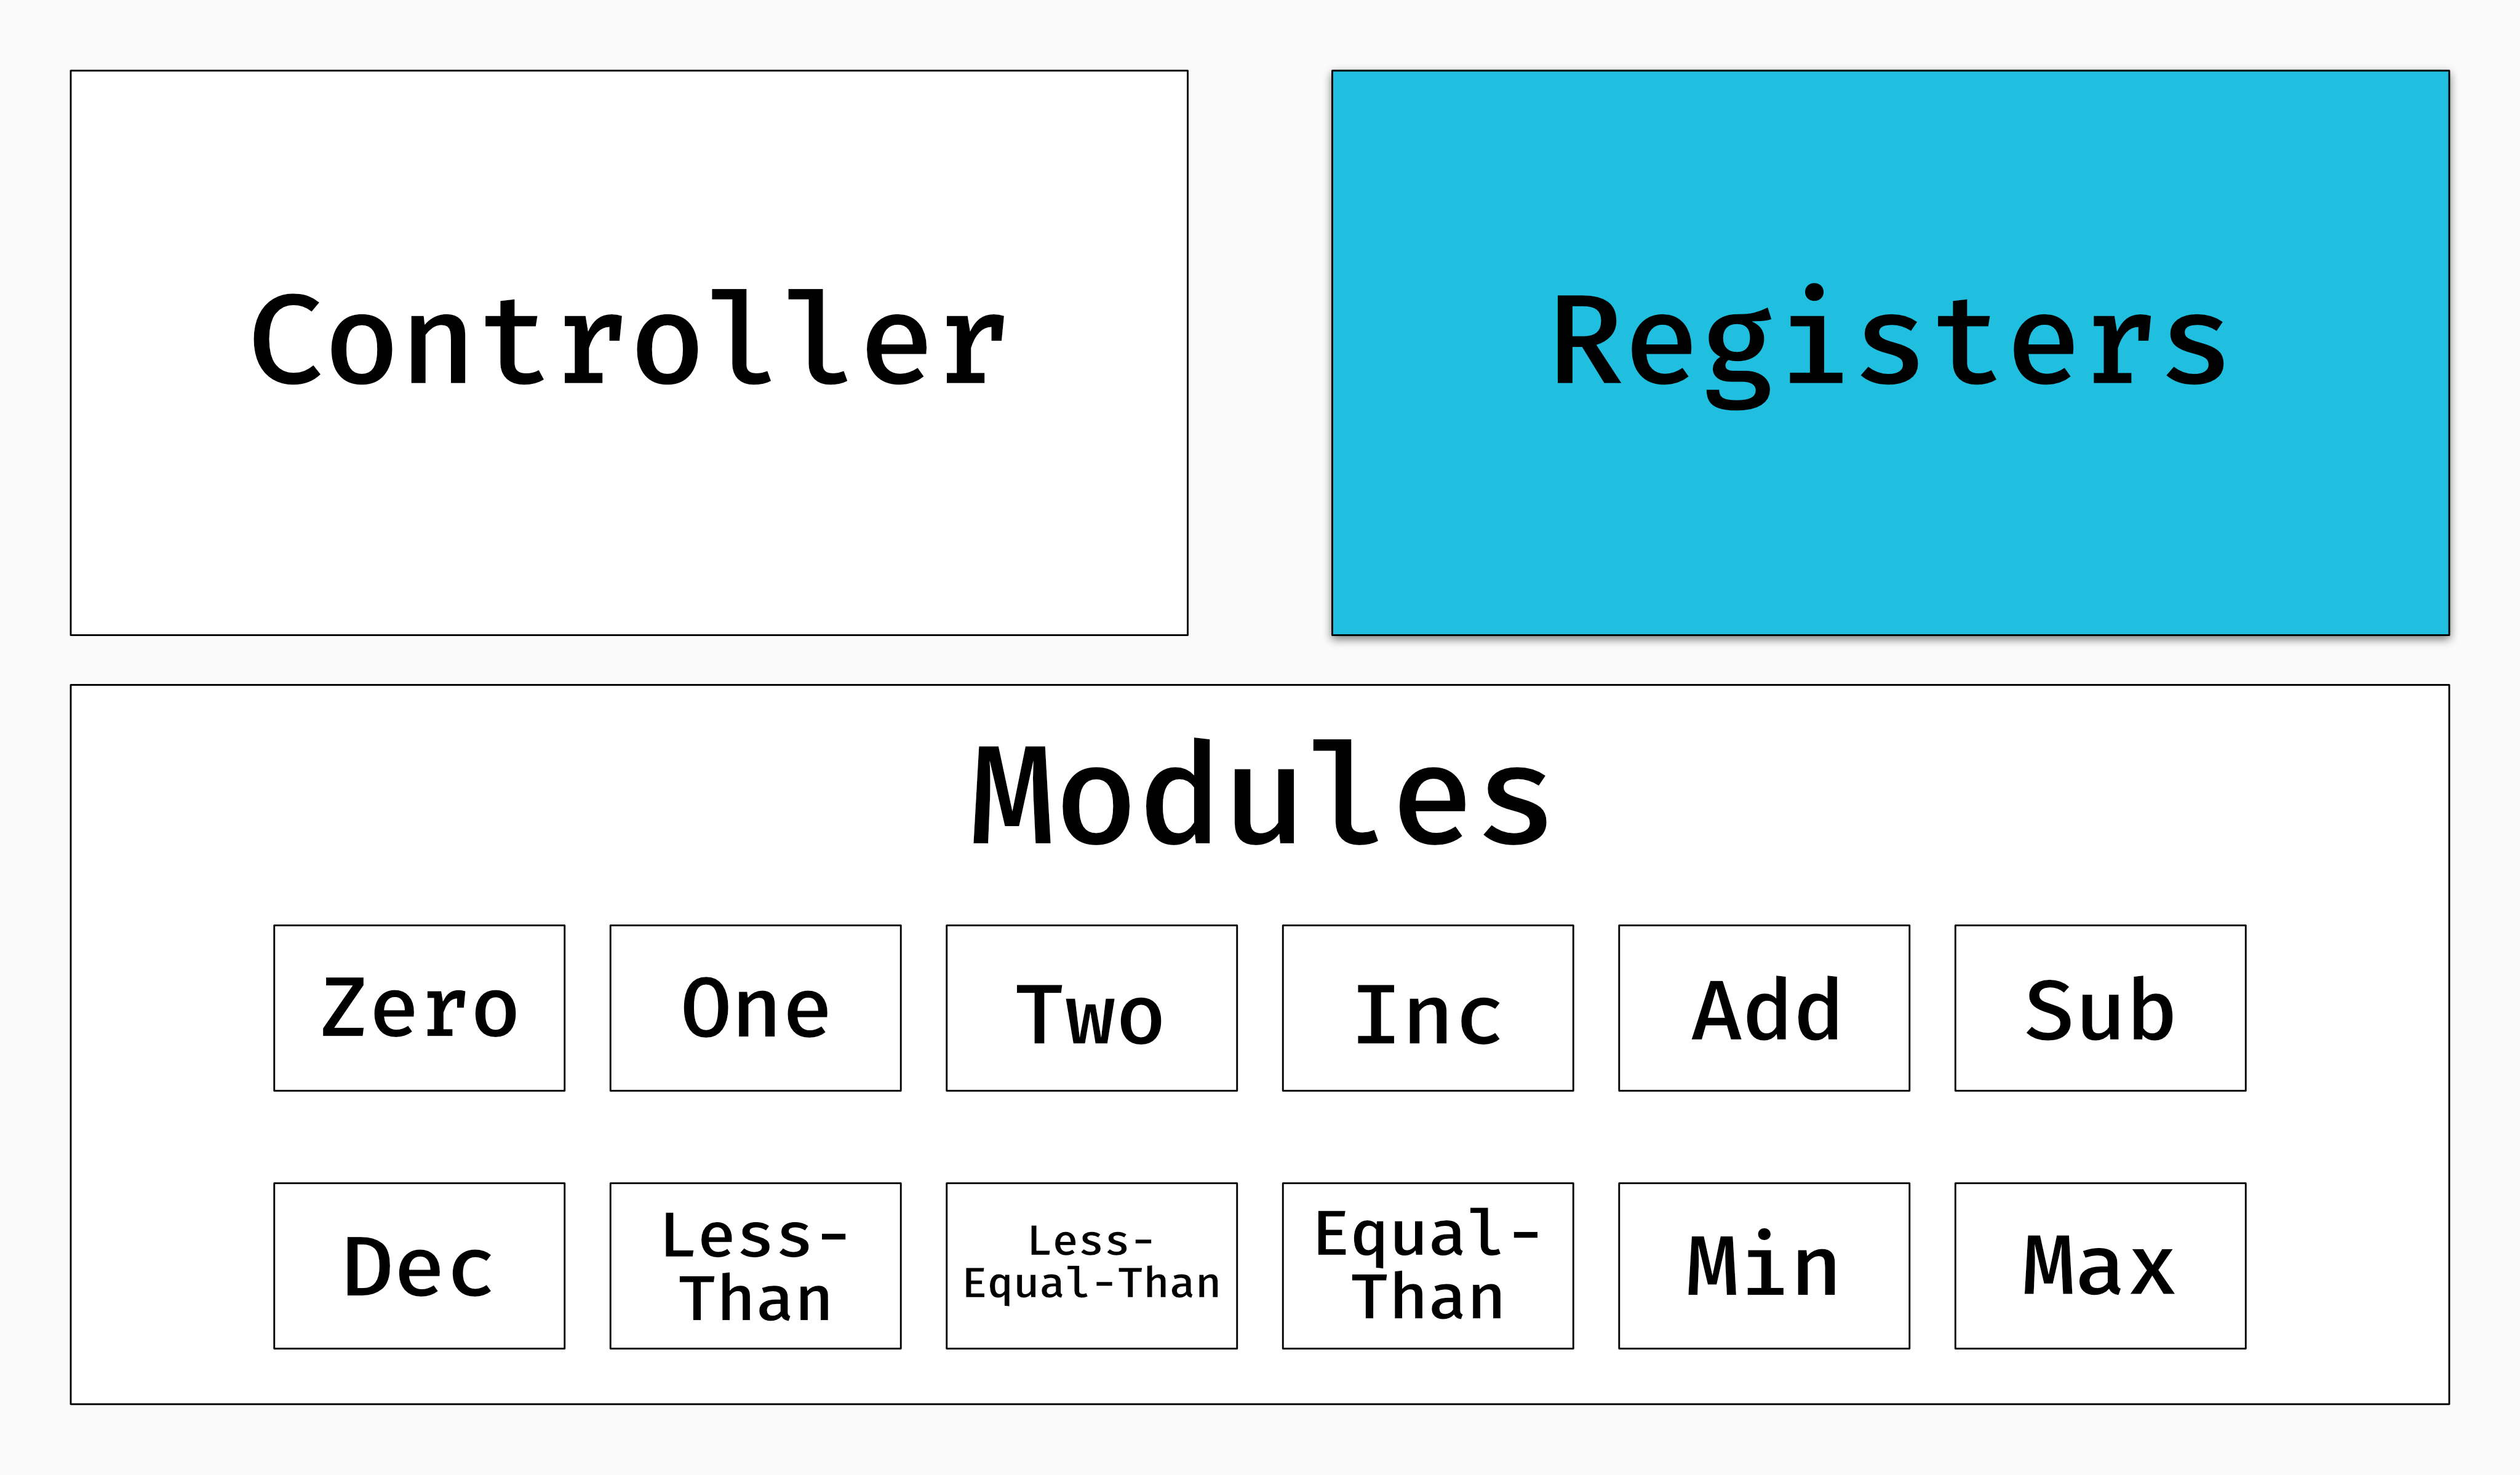
\includegraphics[width=\textwidth]{../figures/schema-nram-without-memory-RS.png}
  	\end{figure}
  \end{frame}
  \begin{frame}{Registers}
  	The registers are a set of memory cells, where each of them contains a probability distribution. Hence, in other words, every register play the role of a random variable.
  \end{frame}
  \begin{frame}{Controller}
  	\begin{figure}
  		\centering
  		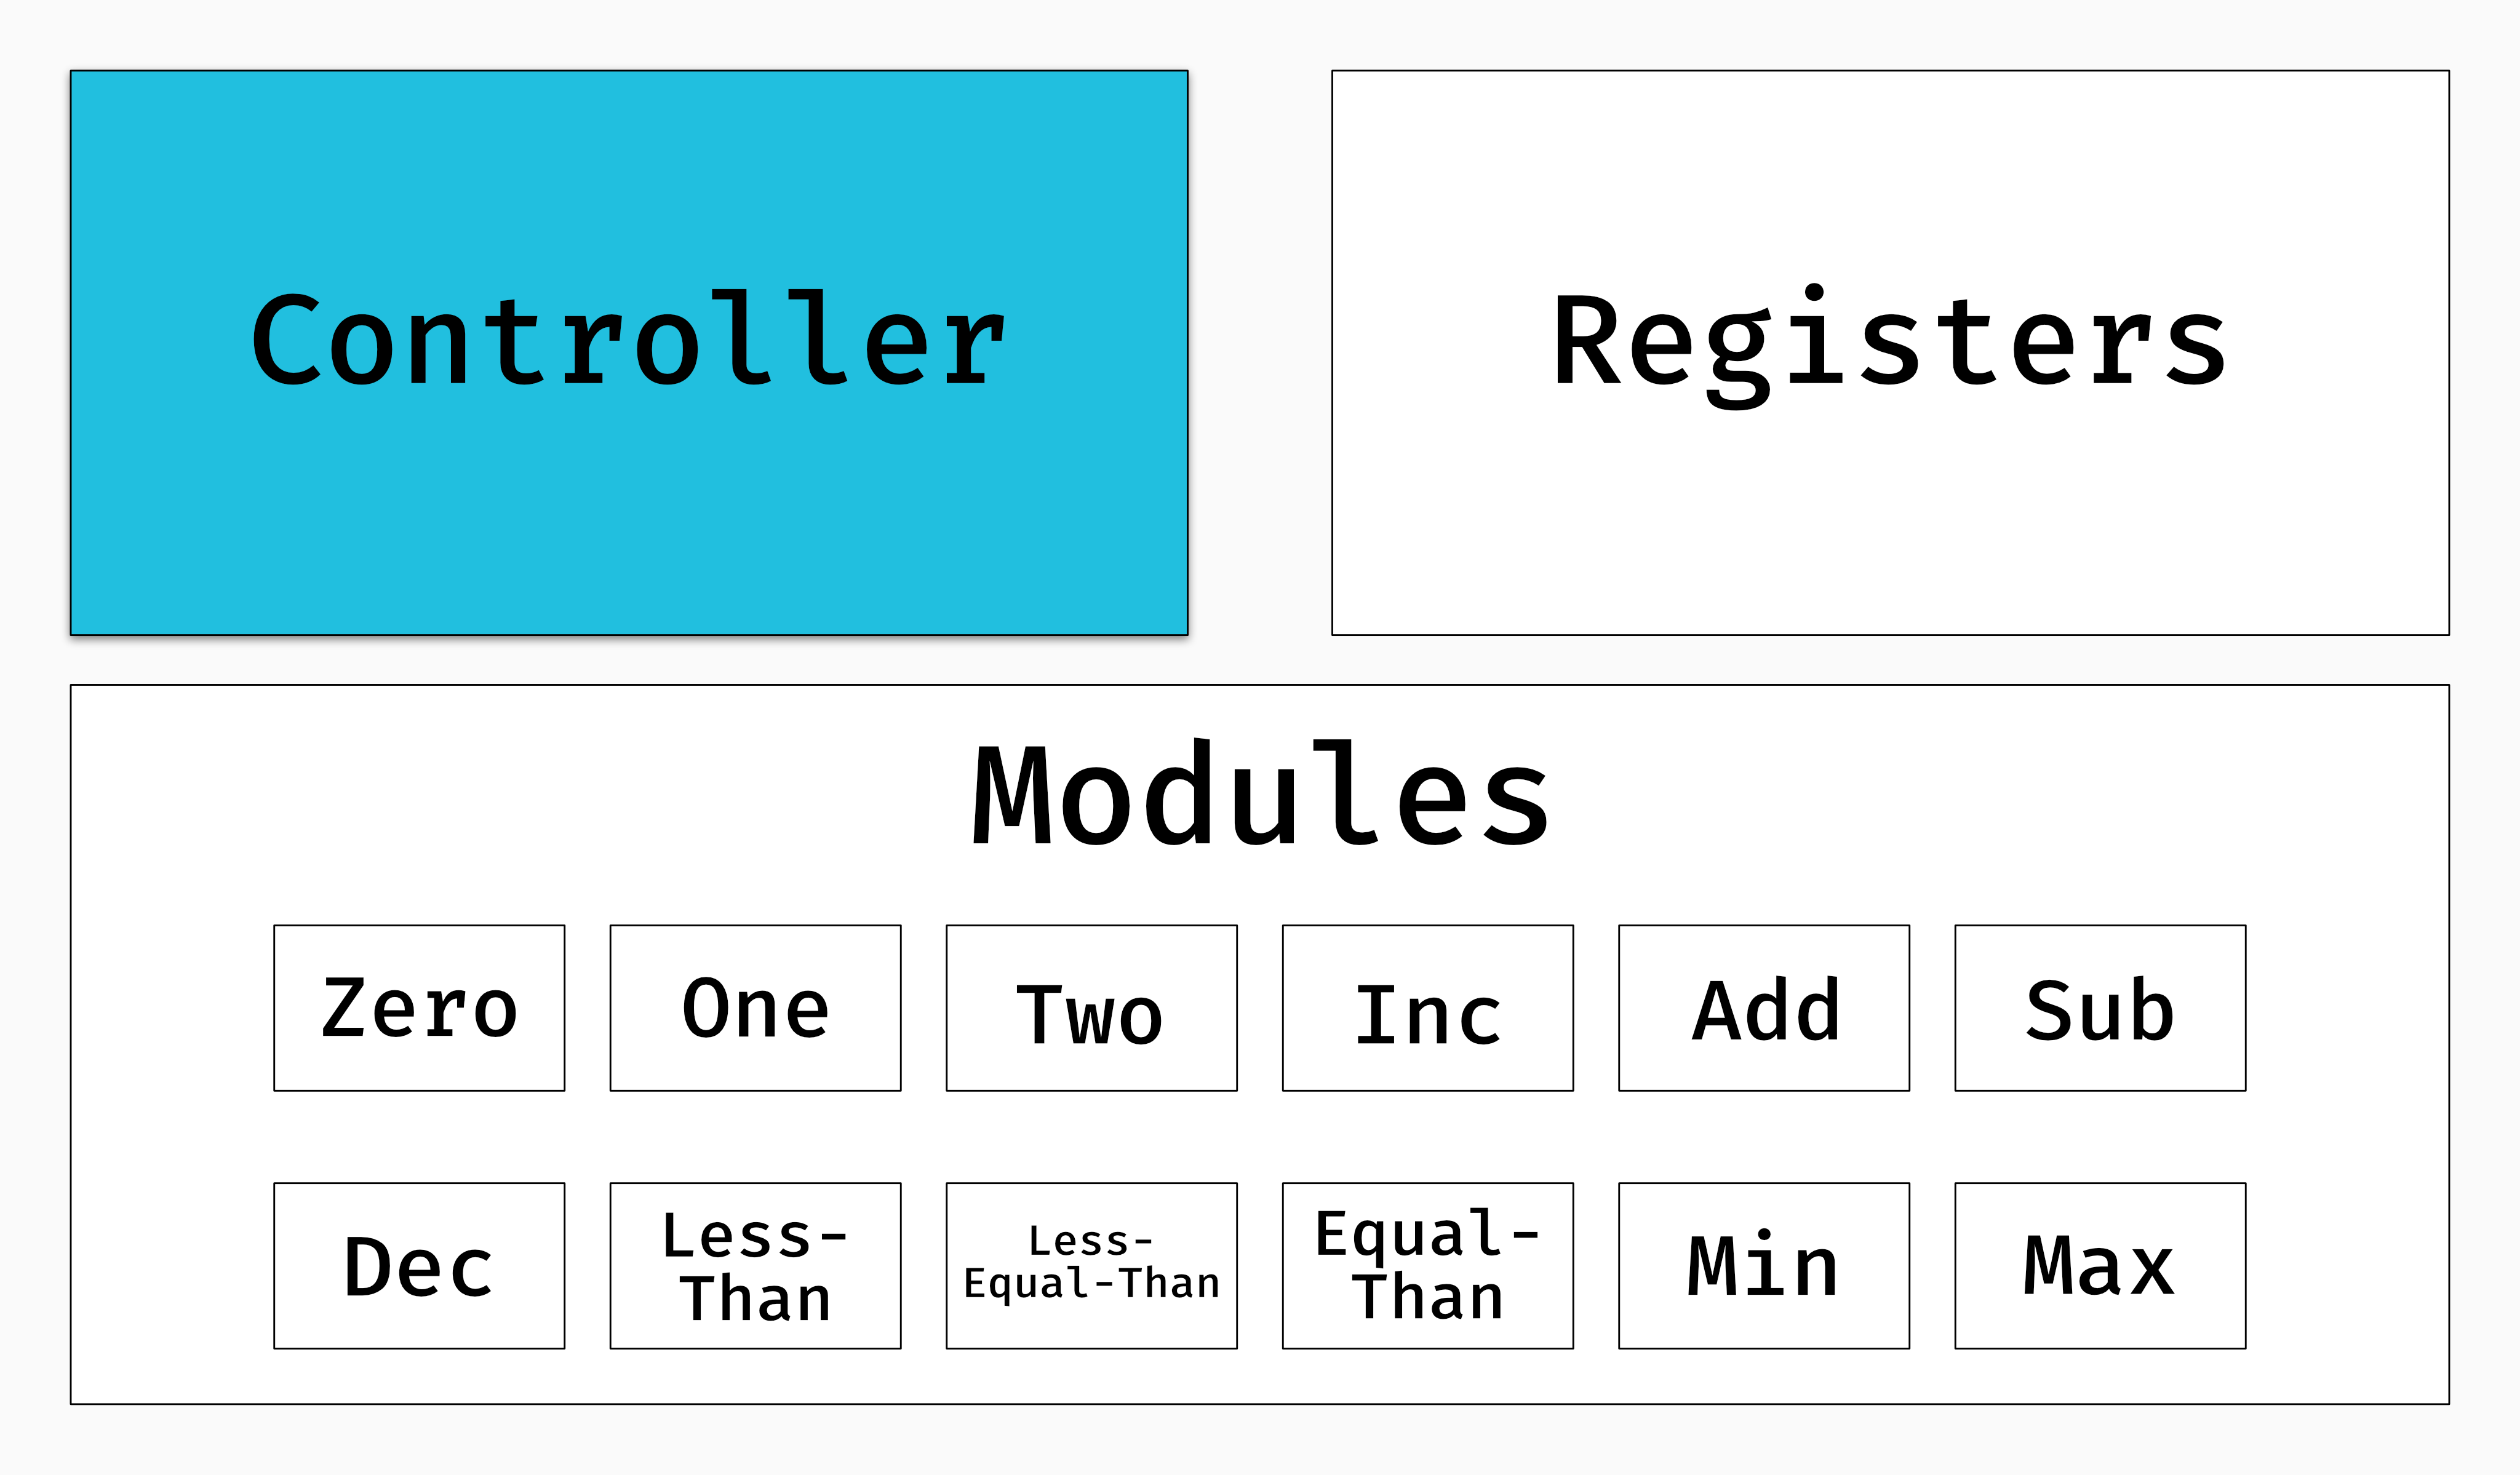
\includegraphics[width=\textwidth]{../figures/schema-nram-without-memory-CL.png}
  	\end{figure}
  \end{frame}
  \begin{frame}{Controller}
  	The controller is a neural network (MLP or LSTM) whose objective is to emit a circuit configuration through which the registers values are manipulated. To do this the controller takes as input the $\mathbb{P}(r_{i} = 0)$ of each register.
  \end{frame}

  \begin{frame}{Timestep execution}  
	\begin{figure}
  		\centering
  		\includegraphics[width=\textwidth]{../figures/timestep.png}
  	\end{figure}
  \end{frame}  
  
  \begin{frame}{Memory augmented version}
  	\begin{figure}
  		\centering
  		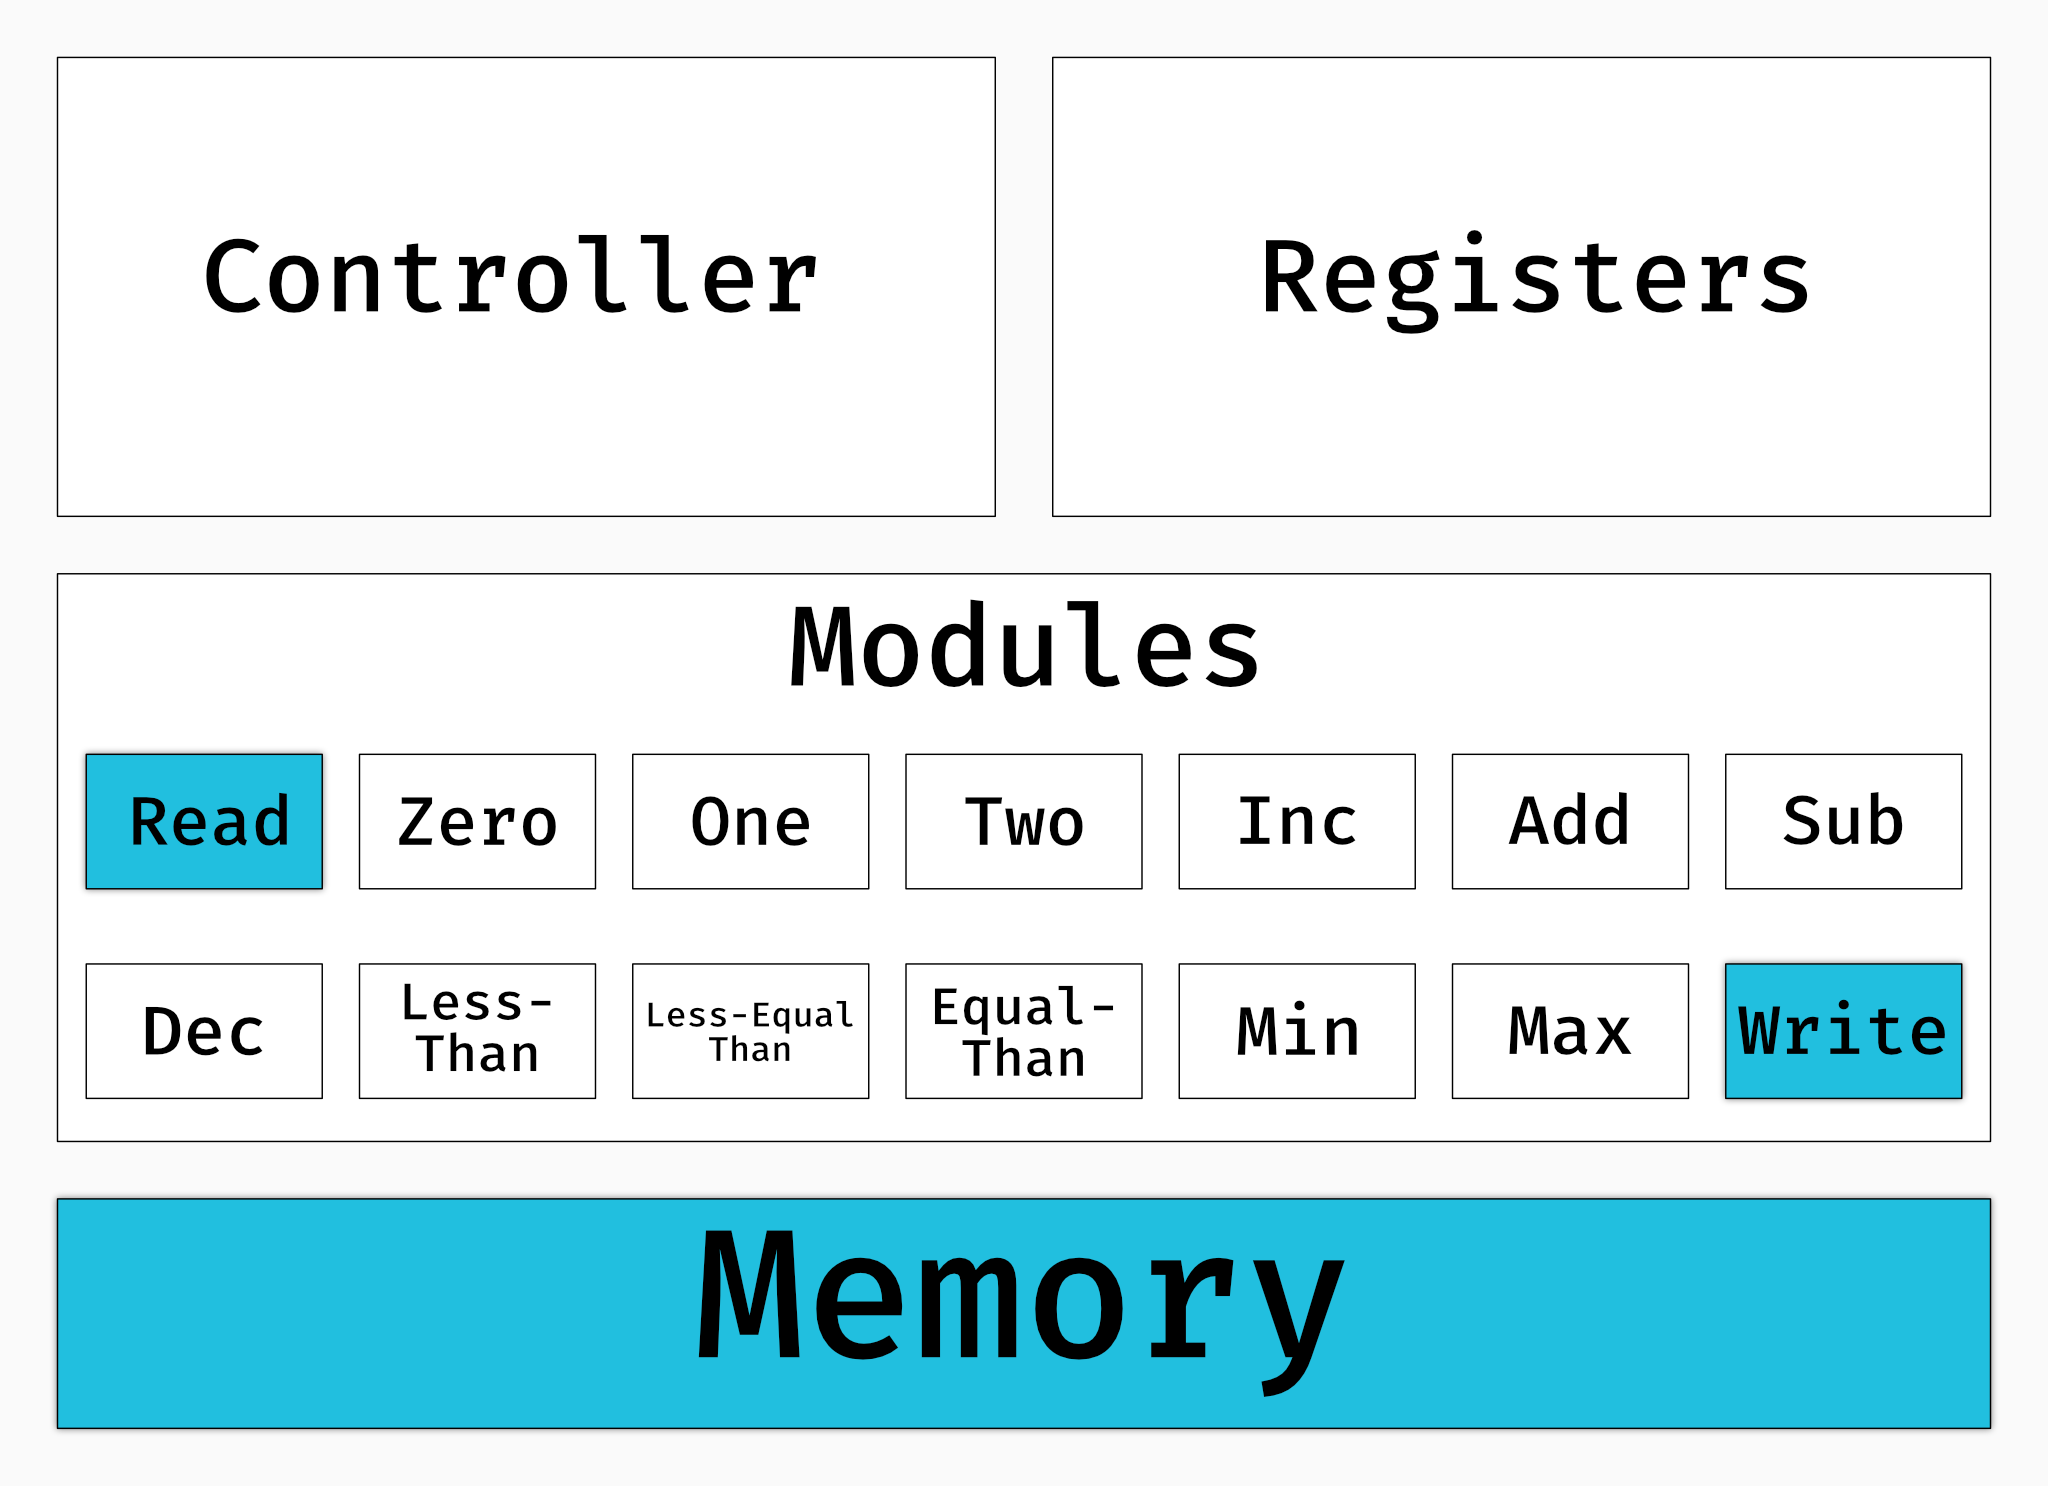
\includegraphics[width=\textwidth]{../figures/schema-nram-with-memory.png}
  	\end{figure}
  \end{frame}
  \begin{frame}{Read \& Write modules}
  
  \end{frame}
  \begin{frame}{Circuit example}
 		
  \end{frame}
  
  \section{Artificial Neural Network}
  \begin{frame}{Description}
  
  \end{frame}
  \begin{frame}{Perceptron}
  	
  \end{frame}
  \begin{frame}{Multi Layer Perceptron (MLP)}
  	
  \end{frame}
  
  \section{Differential Evolution}
  \begin{frame}{Description}
  
  \end{frame}
  \begin{frame}{Differential Evolution variants}
  
  \end{frame}
  \begin{frame}{Mutation variants}
  	
  \end{frame}
  \begin{frame}{Crossover variants}
  	
  \end{frame}
  \begin{frame}{DENN (Differential Evolution for Neural Network)}
  
  \end{frame}
  \section{Implementation and results}
  \begin{frame}{Implementation}
  
  \end{frame}
  \begin{frame}{Results}
  
  \end{frame}
  \begin{frame}{References}
        \bibliography{bibliography}
\end{frame}
\end{document}